%\begin{figure}\center
  %\missingfigure[figheight=.10\textheight, figwidth=\textwidth]{Graphical Abstract}
%  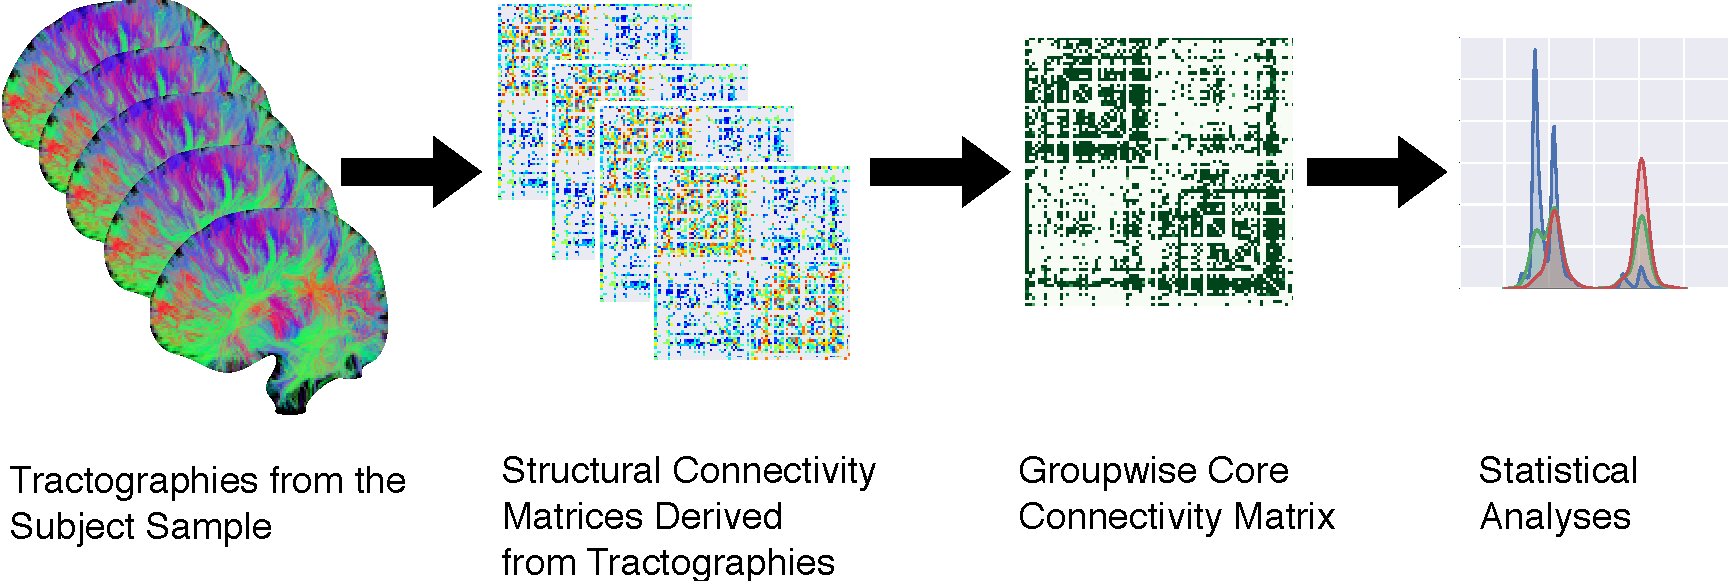
\includegraphics[height=.15\textheight]{graphical_abstract-crop}
%  \caption{Scheme of analyses involving the core structural connectivity matrix.\label{fig:process-illustration}}
%\end{figure}

Isolating the common brain connectivity network from a population is a main problem in current neuroscience~\cite{Bullmore2009,Gong2009,Wassermann2016}. Recent evidence suggests that there's a common and densely connected brain connectome across humans~\cite{Bassett2013}. In this work we present a new approach for selecting these common connections, combining recent topological hypotheses~\cite{Bassett2013}  and  current methods~\cite{Gong2009,Wassermann2016}.

Finding the common brain connectome across subjects has the potential to increase our understanding of the relationship between function and structure in the brain. This relationship is one of the main open questions in neuroscience~\cite{Bullmore2009,Donahue2016}. Moreover, knowledge about the most common connections in a population will facilitate clinical and cognitive Diffusion MRI analyses by reducing the number of surveyed connections, increasing the statistical power of those analyses. Finding the common connectome will also allow us to increase our knowledge about the brain structure by comparing core networks across different populations.

We formalize the problem of selecting the common connections combining graph theory and statistics. Then, we prove that the problem is \NP-Hard and propose a polynomial-time algorithm to find approximate solutions. To do this, we develop an exact polynomial-time algorithm for a relaxed version of the problem and prove the algorithm's correctness and complexity.

Currently, the most used algorithm to extract a population's core structural connectivity network (CSNC)~\cite{Gong2009} uses an statistical approach: first, compute a connectivity matrix for each subject; then, analize each connection separately with a hypothesis test, using as null hypothesis that that edge is not present in the population; finally, construct a binary graph with the edges for which the null hypothesis was rejected. The main problem of Gong et al.'s~\cite{Gong2009} algorithm is that the resulting graph can be a set of disconnected subgraphs. Moreover, recent studies have shown that the brain has a \emph{core} network tightly connected and a sparsely connected \emph{outer} one~\cite{Bassett2013}. In other words, this approach ignores the resulting network's topology. Performing statistical analyses in a feature set chosen by hypothesis testing incurs in the double dipping problem~\cite{Kriegeskorte2009}.

A newer approach to solve the CSNC problem, designed by Wassermann et al.~\cite{Wassermann2016}, uses graph theory to get a connected CSCN: first, compute a binary connectivity graph for each subject using a threshold;  for each possible connection compute the ``cost'' of including or excluding it from the common graph by evaluating in how many subjects that connection is present; finally, construct the binary graph with all the edges that is ``cheaper'' to include than to exclude and connect the resulting graph if it's disconnected, using the minimum possible cost. This algorithm guarantees that the resulting graph is connected, but the connection binarization discards significant information for the resulting common network. In other words, it discards information of the probability of each connection being in the brain. This is problematic because the resulting graph may include edges for which tractography assigned a very low existence probability across subjects. Also, the outer part of the brain, the connections which do not result in the core network, should also be sparsely connected~\cite{Bassett2013}, which this algorithm does not enforce.

In this work we propose, for the first time, a polynomial-time algorithm to obtain the CSCN of a population  addressing the issues listed above. Our algorithm combines the recent graph-theoretical approach~\cite{Wassermann2016} with the statistical awareness of the most popular one~\cite{Gong2009}. We start by formalizing the problem, which allow us to prove that it's \NP-Hard. Then, we propose a first algorithm that solves a relaxed version of the problem in an exact way, giving the best possible core graph for our formalization. Then, we adapt it to guarantee a connected result, agreeing with recent evidence on structural connectivity network topology \cite[e.g.]{Bassett2013}. Finally, we validate our approach using 300 subjects from the HCP database and comparing the performance of the networks obtained by our new approach, Wassermann et al.'s~\cite{Wassermann2016} and Gong et al.'s~\cite{Gong2009} predicting connectivity values from handedness in the core network.